\chapter{Technical Implementation and AI Integration}

\section{BCD.NET Platform Architecture}

\subsection{Platform Overview}
The BCD.NET platform represents a comprehensive digital transformation of BCD's networking capabilities, designed to enhance member engagement, facilitate deal flow, and provide intelligent matching services. The platform integrates modern web technologies with AI-powered features to create a seamless networking experience.

\begin{figure}[h]
\centering
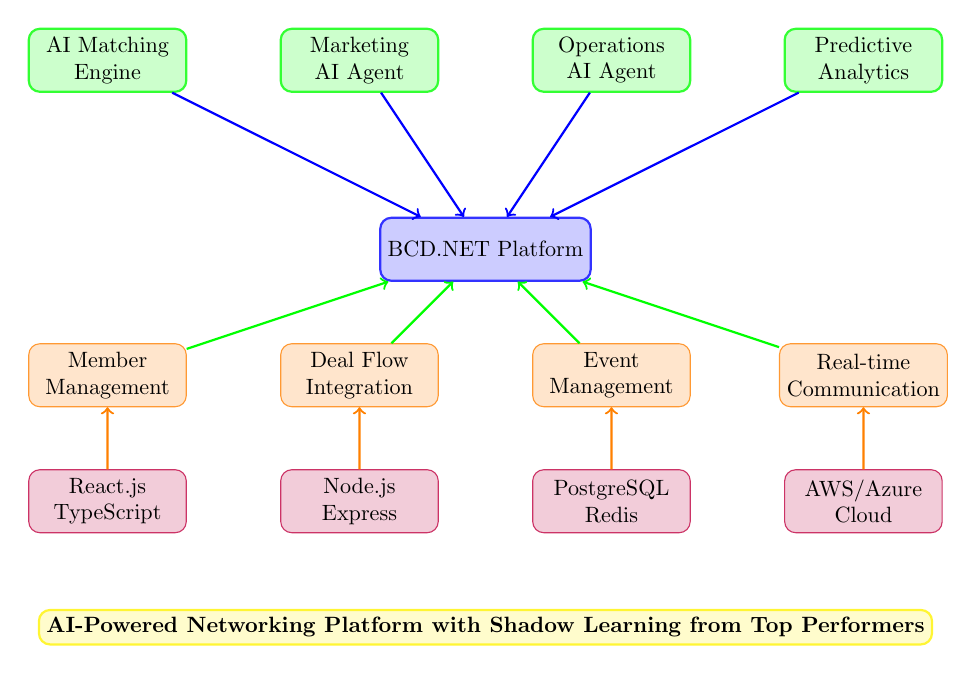
\begin{tikzpicture}[
    scale=0.8,
    transform shape,
    box/.style={rectangle, draw, rounded corners, minimum width=2.5cm, minimum height=1cm, align=center},
    platform/.style={box, fill=blue!20, draw=blue!80, thick},
    ai/.style={box, fill=green!20, draw=green!80, thick},
    feature/.style={box, fill=orange!20, draw=orange!80},
    tech/.style={box, fill=purple!20, draw=purple!80},
    arrow/.style={->, thick}
]

% Core Platform
\node[platform] (bcd) at (0,0) {BCD.NET Platform};

% AI Components
\node[ai] (matching) at (-6,3) {AI Matching\\Engine};
\node[ai] (marketing) at (-2,3) {Marketing\\AI Agent};
\node[ai] (operations) at (2,3) {Operations\\AI Agent};
\node[ai] (analytics) at (6,3) {Predictive\\Analytics};

% Core Features
\node[feature] (members) at (-6,-2) {Member\\Management};
\node[feature] (deals) at (-2,-2) {Deal Flow\\Integration};
\node[feature] (events) at (2,-2) {Event\\Management};
\node[feature] (communication) at (6,-2) {Real-time\\Communication};

% Technology Stack
\node[tech] (frontend) at (-6,-4) {React.js\\TypeScript};
\node[tech] (backend) at (-2,-4) {Node.js\\Express};
\node[tech] (database) at (2,-4) {PostgreSQL\\Redis};
\node[tech] (cloud) at (6,-4) {AWS/Azure\\Cloud};

% Connections
\draw[arrow, blue] (matching) -- (bcd);
\draw[arrow, blue] (marketing) -- (bcd);
\draw[arrow, blue] (operations) -- (bcd);
\draw[arrow, blue] (analytics) -- (bcd);

\draw[arrow, green] (members) -- (bcd);
\draw[arrow, green] (deals) -- (bcd);
\draw[arrow, green] (events) -- (bcd);
\draw[arrow, green] (communication) -- (bcd);

\draw[arrow, orange] (frontend) -- (members);
\draw[arrow, orange] (backend) -- (deals);
\draw[arrow, orange] (database) -- (events);
\draw[arrow, orange] (cloud) -- (communication);

% Platform highlights
\node[fill=yellow!20, draw=yellow!80, thick, rounded corners] at (0,-6) 
    {\textbf{AI-Powered Networking Platform with Shadow Learning from Top Performers}};

\end{tikzpicture}
\caption{BCD.NET Platform Architecture and AI Integration}
\label{fig:bcd-platform-architecture}
\end{figure}

\subsection{Technical Architecture}
\begin{itemize}
    \item \textbf{Frontend}: React.js with TypeScript for robust user interface
    \item \textbf{Backend}: Node.js with Express.js for scalable API development
    \item \textbf{Database}: PostgreSQL for relational data with Redis for caching
    \item \textbf{Authentication}: JWT-based secure authentication system
    \item \textbf{Real-time Communication}: WebSocket integration for instant messaging
    \item \textbf{Cloud Infrastructure}: AWS or Azure for scalable deployment
\end{itemize}

\subsection{Core Platform Features}
\subsubsection{Member Management System}
\begin{itemize}
    \item Comprehensive member profiles with verification processes
    \item Advanced search and filtering capabilities
    \item Privacy controls and data protection compliance
    \item Integration with existing WhatsApp community
    \item Member activity tracking and engagement analytics
\end{itemize}

\subsubsection{Deal Flow Integration}
\begin{itemize}
    \item Deal posting and discovery system
    \item Investment opportunity matching
    \item Due diligence document sharing
    \item Deal tracking and status updates
    \item Investment syndicate formation tools
\end{itemize}

\subsubsection{Event Management}
\begin{itemize}
    \item Event creation and registration system
    \item Calendar integration and notifications
    \item Attendee management and networking facilitation
    \item Post-event feedback and analytics
    \item Hybrid event support (virtual and physical)
\end{itemize}

\section{AI Agent-Based Pairing Mechanism}

\subsection{Intelligent Matching Algorithm}
The AI-powered pairing system represents a breakthrough in networking efficiency, designed to facilitate meaningful connections based on multiple criteria beyond simple industry matching.

\subsubsection{Matching Criteria}
\begin{itemize}
    \item \textbf{Business Profile}: Company size, industry, growth stage
    \item \textbf{Investment Interests}: Deal flow preferences, investment thesis
    \item \textbf{Geographic Focus}: Regional expertise and market knowledge
    \item \textbf{Professional Background}: Experience level, expertise areas
    \item \textbf{Networking Goals}: Specific objectives and desired outcomes
    \item \textbf{Compatibility Factors}: Communication style, meeting preferences
\end{itemize}

\subsubsection{AI Algorithm Components}
\begin{itemize}
    \item \textbf{Machine Learning Models}: Supervised learning for connection success prediction
    \item \textbf{Natural Language Processing}: Analysis of member profiles and preferences
    \item \textbf{Recommendation Engine}: Collaborative filtering and content-based filtering
    \item \textbf{Real-time Learning}: Continuous improvement based on user feedback
    \item \textbf{Privacy-Preserving Matching}: Secure data handling and anonymization
\end{itemize}

\subsection{Shadow Learning from Top Performers}
The most effective AI agent development strategy involves shadowing top performers and codifying their decision-making processes into concrete, actionable frameworks.

\begin{figure}[h]
\centering
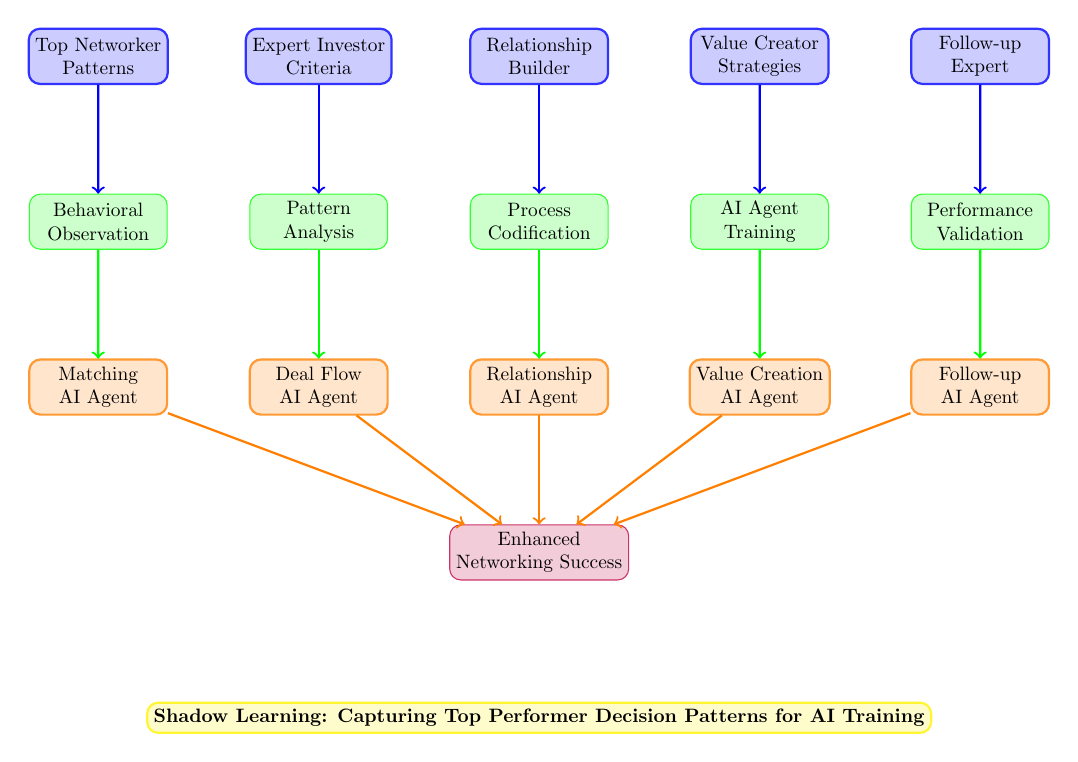
\begin{tikzpicture}[
    scale=0.7,
    transform shape,
    box/.style={rectangle, draw, rounded corners, minimum width=2.5cm, minimum height=1cm, align=center},
    performer/.style={box, fill=blue!20, draw=blue!80, thick},
    process/.style={box, fill=green!20, draw=green!80},
    ai/.style={box, fill=orange!20, draw=orange!80, thick},
    outcome/.style={box, fill=purple!20, draw=purple!80},
    arrow/.style={->, thick}
]

% Top Performers
\node[performer] (networker) at (-8,4) {Top Networker\\Patterns};
\node[performer] (investor) at (-4,4) {Expert Investor\\Criteria};
\node[performer] (relationship) at (0,4) {Relationship\\Builder};
\node[performer] (value) at (4,4) {Value Creator\\Strategies};
\node[performer] (followup) at (8,4) {Follow-up\\Expert};

% Learning Process
\node[process] (observation) at (-8,1) {Behavioral\\Observation};
\node[process] (analysis) at (-4,1) {Pattern\\Analysis};
\node[process] (codification) at (0,1) {Process\\Codification};
\node[process] (training) at (4,1) {AI Agent\\Training};
\node[process] (validation) at (8,1) {Performance\\Validation};

% AI Agents
\node[ai] (matching_ai) at (-8,-2) {Matching\\AI Agent};
\node[ai] (deal_ai) at (-4,-2) {Deal Flow\\AI Agent};
\node[ai] (relationship_ai) at (0,-2) {Relationship\\AI Agent};
\node[ai] (value_ai) at (4,-2) {Value Creation\\AI Agent};
\node[ai] (followup_ai) at (8,-2) {Follow-up\\AI Agent};

% Outcomes
\node[outcome] (success) at (0,-5) {Enhanced\\Networking Success};

% Learning flow
\draw[arrow, blue] (networker) -- (observation);
\draw[arrow, blue] (investor) -- (analysis);
\draw[arrow, blue] (relationship) -- (codification);
\draw[arrow, blue] (value) -- (training);
\draw[arrow, blue] (followup) -- (validation);

% Process flow
\draw[arrow, green] (observation) -- (matching_ai);
\draw[arrow, green] (analysis) -- (deal_ai);
\draw[arrow, green] (codification) -- (relationship_ai);
\draw[arrow, green] (training) -- (value_ai);
\draw[arrow, green] (validation) -- (followup_ai);

% AI outcomes
\draw[arrow, orange] (matching_ai) -- (success);
\draw[arrow, orange] (deal_ai) -- (success);
\draw[arrow, orange] (relationship_ai) -- (success);
\draw[arrow, orange] (value_ai) -- (success);
\draw[arrow, orange] (followup_ai) -- (success);

% Shadow learning highlight
\node[fill=yellow!20, draw=yellow!80, thick, rounded corners] at (0,-8) 
    {\textbf{Shadow Learning: Capturing Top Performer Decision Patterns for AI Training}};

\end{tikzpicture}
\caption{AI Agent Shadow Learning Process from Top Performers}
\label{fig:shadow-learning-process}
\end{figure}

\subsubsection{Top Performer Analysis}
\begin{itemize}
    \item \textbf{Network Building Patterns}: How successful members identify and approach potential connections
    \item \textbf{Deal Flow Assessment}: Criteria used by experienced investors to evaluate opportunities
    \item \textbf{Relationship Development}: Strategies for building and maintaining professional relationships
    \item \textbf{Value Creation}: Methods for creating mutual value in networking interactions
    \item \textbf{Follow-up Strategies}: Systematic approaches to maintaining connection momentum
\end{itemize}

\subsubsection{AI Agent Training Framework}
\begin{itemize}
    \item \textbf{Behavioral Modeling}: Capturing decision patterns from successful networkers
    \item \textbf{Scenario Training}: Teaching AI agents to handle various networking situations
    \item \textbf{Feedback Integration}: Continuous learning from member interactions and outcomes
    \item \textbf{Ethical Guidelines}: Ensuring AI recommendations align with BCD's values
    \item \textbf{Performance Metrics}: Measuring AI agent effectiveness in facilitating successful connections
\end{itemize}

\section{AI-Powered Business Operations}

\subsection{Marketing Strategy AI Agent}
The development of AI agents for marketing strategy represents a significant opportunity to enhance BCD's competitive positioning and growth initiatives.

\subsubsection{Market Intelligence Analysis}
\begin{itemize}
    \item \textbf{Competitive Monitoring}: Automated tracking of competitor activities and positioning
    \item \textbf{Market Trend Analysis}: Real-time identification of emerging opportunities and threats
    \item \textbf{Member Sentiment Analysis}: Understanding member needs and satisfaction levels
    \item \textbf{Content Performance Optimization}: AI-driven content strategy and optimization
    \item \textbf{Lead Generation Intelligence}: Identifying high-potential prospects and engagement opportunities
\end{itemize}

\subsubsection{Personalized Marketing Automation}
\begin{itemize}
    \item \textbf{Member Segmentation}: AI-powered member categorization and targeting
    \item \textbf{Content Personalization}: Tailored messaging and content delivery
    \item \textbf{Engagement Optimization}: Automated follow-up and relationship nurturing
    \item \textbf{Event Recommendation}: Intelligent suggestions for member participation
    \item \textbf{Referral Optimization}: AI-enhanced member referral program management
\end{itemize}

\subsection{Business Operations AI Agent}
AI agents can significantly enhance BCD's operational efficiency and decision-making processes.

\subsubsection{Operational Intelligence}
\begin{itemize}
    \item \textbf{Performance Analytics}: Real-time monitoring of key business metrics
    \item \textbf{Predictive Modeling}: Forecasting member growth, retention, and revenue trends
    \item \textbf{Resource Optimization}: AI-driven allocation of marketing and operational resources
    \item \textbf{Risk Assessment}: Automated identification of potential business risks and opportunities
    \item \textbf{Process Automation}: Streamlining repetitive operational tasks
\end{itemize}

\subsubsection{Strategic Decision Support}
\begin{itemize}
    \item \textbf{Market Entry Analysis}: AI-powered evaluation of expansion opportunities
    \item \textbf{Partnership Assessment}: Automated analysis of potential strategic partnerships
    \item \textbf{Investment Prioritization}: AI-driven resource allocation for platform development
    \item \textbf{Competitive Response Planning}: Automated monitoring and response to competitive threats
    \item \textbf{Scenario Planning}: AI-powered modeling of different business scenarios and outcomes
\end{itemize}

\section{Implementation Roadmap}

\subsection{Phase 1: Foundation (Months 1-6)}
\begin{itemize}
    \item \textbf{Platform Development}: Core BCD.NET platform with basic member management
    \item \textbf{Data Infrastructure}: Secure data collection and storage systems
    \item \textbf{Basic AI Integration}: Simple recommendation algorithms and matching
    \item \textbf{User Testing}: Member feedback and platform optimization
    \item \textbf{Security Implementation}: Comprehensive data protection and privacy measures
\end{itemize}

\subsection{Phase 2: AI Enhancement (Months 7-18)}
\begin{itemize}
    \item \textbf{Advanced Matching}: Sophisticated AI-powered pairing algorithms
    \item \textbf{Marketing AI}: Automated marketing strategy and content optimization
    \item \textbf{Operational AI}: Business intelligence and decision support systems
    \item \textbf{Mobile Application}: Native mobile app for enhanced user experience
    \item \textbf{API Integration}: Third-party service integrations and partnerships
\end{itemize}

\subsection{Phase 3: Advanced Features (Months 19-36)}
\begin{itemize}
    \item \textbf{Predictive Analytics}: Advanced forecasting and trend analysis
    \item \textbf{Automated Deal Flow}: AI-powered deal discovery and matching
    \item \textbf{Virtual Events Platform}: Comprehensive hybrid event management
    \item \textbf{Advanced Security}: Blockchain-based verification and trust systems
    \item \textbf{Global Expansion}: Multi-language and multi-region platform support
\end{itemize}

\section{Technical Considerations}

\subsection{Scalability and Performance}
\begin{itemize}
    \item \textbf{Microservices Architecture}: Modular design for easy scaling and maintenance
    \item \textbf{Cloud-Native Development}: Containerized deployment for flexibility
    \item \textbf{Database Optimization}: Efficient data storage and retrieval systems
    \item \textbf{CDN Integration}: Global content delivery for optimal performance
    \item \textbf{Load Balancing}: Automated traffic distribution and failover systems
\end{itemize}

\subsection{Security and Privacy}
\begin{itemize}
    \item \textbf{Data Encryption}: End-to-end encryption for sensitive information
    \item \textbf{GDPR Compliance}: Full compliance with European data protection regulations
    \item \textbf{Access Control}: Role-based permissions and authentication
    \item \textbf{Audit Trails}: Comprehensive logging and monitoring systems
    \item \textbf{Regular Security Audits}: Ongoing vulnerability assessment and remediation
\end{itemize}

\subsection{AI Ethics and Governance}
\begin{itemize}
    \item \textbf{Transparency}: Clear explanation of AI decision-making processes
    \item \textbf{Fairness}: Ensuring AI algorithms don't perpetuate biases
    \item \textbf{Accountability}: Human oversight and control of AI systems
    \item \textbf{Privacy Protection}: Minimizing data collection and ensuring user control
    \item \textbf{Continuous Monitoring}: Regular assessment of AI system performance and impact
\end{itemize}

\section{Success Metrics and KPIs}

\subsection{Platform Performance Metrics}
\begin{itemize}
    \item \textbf{User Engagement}: Daily active users, session duration, feature adoption
    \item \textbf{Connection Success Rate}: Percentage of AI-suggested connections that result in meaningful interactions
    \item \textbf{Platform Reliability}: Uptime, response time, error rates
    \item \textbf{Member Satisfaction}: Net Promoter Score and user feedback scores
    \item \textbf{Deal Flow Integration}: Number of deals posted and successfully matched
\end{itemize}

\subsection{AI Effectiveness Metrics}
\begin{itemize}
    \item \textbf{Matching Accuracy}: Success rate of AI-powered connection suggestions
    \item \textbf{Learning Efficiency}: Rate of AI model improvement over time
    \item \textbf{User Adoption}: Percentage of members using AI-powered features
    \item \textbf{Business Impact}: Correlation between AI usage and member success metrics
    \item \textbf{Ethical Compliance}: Monitoring for bias and fairness in AI recommendations
\end{itemize}

\section{Investment Requirements}

\subsection{Development Costs}
\begin{itemize}
    \item \textbf{Platform Development}: €500,000 - €1,000,000 for full-featured platform
    \item \textbf{AI Integration}: €200,000 - €400,000 for advanced AI capabilities
    \item \textbf{Security Implementation}: €100,000 - €200,000 for comprehensive security
    \item \textbf{Testing and Quality Assurance}: €150,000 - €300,000 for thorough testing
    \item \textbf{Deployment and Infrastructure}: €100,000 - €200,000 for cloud infrastructure
\end{itemize}

\subsection{Ongoing Operational Costs}
\begin{itemize}
    \item \textbf{Platform Maintenance}: €50,000 - €100,000 annually
    \item \textbf{AI Model Training}: €30,000 - €60,000 annually
    \item \textbf{Security Monitoring}: €20,000 - €40,000 annually
    \item \textbf{Cloud Infrastructure}: €40,000 - €80,000 annually
    \item \textbf{Technical Support}: €30,000 - €60,000 annually
\end{itemize}

The technical implementation of BCD.NET with AI integration represents a significant competitive advantage, enabling BCD to provide unparalleled networking experiences while maintaining the human touch that defines premium networking platforms. The shadow learning approach ensures that AI agents capture the nuanced decision-making processes of top performers, creating a powerful combination of human expertise and artificial intelligence. 